\documentclass[twoside]{book}

% Packages required by doxygen
\usepackage{fixltx2e}
\usepackage{calc}
\usepackage{doxygen}
\usepackage[export]{adjustbox} % also loads graphicx
\usepackage{graphicx}
\usepackage[utf8]{inputenc}
\usepackage{makeidx}
\usepackage{multicol}
\usepackage{multirow}
\PassOptionsToPackage{warn}{textcomp}
\usepackage{textcomp}
\usepackage[nointegrals]{wasysym}
\usepackage[table]{xcolor}

% Font selection
\usepackage[T1]{fontenc}
\usepackage[scaled=.90]{helvet}
\usepackage{courier}
\usepackage{amssymb}
\usepackage{sectsty}
\renewcommand{\familydefault}{\sfdefault}
\allsectionsfont{%
  \fontseries{bc}\selectfont%
  \color{darkgray}%
}
\renewcommand{\DoxyLabelFont}{%
  \fontseries{bc}\selectfont%
  \color{darkgray}%
}
\newcommand{\+}{\discretionary{\mbox{\scriptsize$\hookleftarrow$}}{}{}}

% Page & text layout
\usepackage{geometry}
\geometry{%
  a4paper,%
  top=2.5cm,%
  bottom=2.5cm,%
  left=2.5cm,%
  right=2.5cm%
}
\tolerance=750
\hfuzz=15pt
\hbadness=750
\setlength{\emergencystretch}{15pt}
\setlength{\parindent}{0cm}
\setlength{\parskip}{3ex plus 2ex minus 2ex}
\makeatletter
\renewcommand{\paragraph}{%
  \@startsection{paragraph}{4}{0ex}{-1.0ex}{1.0ex}{%
    \normalfont\normalsize\bfseries\SS@parafont%
  }%
}
\renewcommand{\subparagraph}{%
  \@startsection{subparagraph}{5}{0ex}{-1.0ex}{1.0ex}{%
    \normalfont\normalsize\bfseries\SS@subparafont%
  }%
}
\makeatother

% Headers & footers
\usepackage{fancyhdr}
\pagestyle{fancyplain}
\fancyhead[LE]{\fancyplain{}{\bfseries\thepage}}
\fancyhead[CE]{\fancyplain{}{}}
\fancyhead[RE]{\fancyplain{}{\bfseries\leftmark}}
\fancyhead[LO]{\fancyplain{}{\bfseries\rightmark}}
\fancyhead[CO]{\fancyplain{}{}}
\fancyhead[RO]{\fancyplain{}{\bfseries\thepage}}
\fancyfoot[LE]{\fancyplain{}{}}
\fancyfoot[CE]{\fancyplain{}{}}
\fancyfoot[RE]{\fancyplain{}{\bfseries\scriptsize Generated by Doxygen }}
\fancyfoot[LO]{\fancyplain{}{\bfseries\scriptsize Generated by Doxygen }}
\fancyfoot[CO]{\fancyplain{}{}}
\fancyfoot[RO]{\fancyplain{}{}}
\renewcommand{\footrulewidth}{0.4pt}
\renewcommand{\chaptermark}[1]{%
  \markboth{#1}{}%
}
\renewcommand{\sectionmark}[1]{%
  \markright{\thesection\ #1}%
}

% Indices & bibliography
\usepackage{natbib}
\usepackage[titles]{tocloft}
\setcounter{tocdepth}{3}
\setcounter{secnumdepth}{5}
\makeindex

% Hyperlinks (required, but should be loaded last)
\usepackage{ifpdf}
\ifpdf
  \usepackage[pdftex,pagebackref=true]{hyperref}
\else
  \usepackage[ps2pdf,pagebackref=true]{hyperref}
\fi
\hypersetup{%
  colorlinks=true,%
  linkcolor=blue,%
  citecolor=blue,%
  unicode%
}

% Custom commands
\newcommand{\clearemptydoublepage}{%
  \newpage{\pagestyle{empty}\cleardoublepage}%
}

\usepackage{caption}
\captionsetup{labelsep=space,justification=centering,font={bf},singlelinecheck=off,skip=4pt,position=top}

%===== C O N T E N T S =====

\begin{document}

% Titlepage & ToC
\hypersetup{pageanchor=false,
             bookmarksnumbered=true,
             pdfencoding=unicode
            }
\pagenumbering{roman}
\begin{titlepage}
\vspace*{7cm}
\begin{center}%
{\Large My Project }\\
\vspace*{1cm}
{\large Generated by Doxygen 1.8.11}\\
\end{center}
\end{titlepage}
\clearemptydoublepage
\tableofcontents
\clearemptydoublepage
\pagenumbering{arabic}
\hypersetup{pageanchor=true}

%--- Begin generated contents ---
\chapter{Class Index}
\section{Class List}
Here are the classes, structs, unions and interfaces with brief descriptions\+:\begin{DoxyCompactList}
\item\contentsline{section}{\hyperlink{classRobot}{Robot} \\*\hyperlink{classRobot}{Robot} class responsible for running yolov3 on image or video }{\pageref{classRobot}}{}
\item\contentsline{section}{\hyperlink{classUtils}{Utils} \\*\hyperlink{classUtils}{Utils} class used in \hyperlink{classYOLOv3}{Y\+O\+L\+Ov3} class for configuring the cv\+::dnn\+::\+Net }{\pageref{classUtils}}{}
\item\contentsline{section}{\hyperlink{classYOLOv3}{Y\+O\+L\+Ov3} \\*\hyperlink{classYOLOv3}{Y\+O\+L\+Ov3} class responsible for running object detection on image or video }{\pageref{classYOLOv3}}{}
\end{DoxyCompactList}

\chapter{File Index}
\section{File List}
Here is a list of all documented files with brief descriptions\+:\begin{DoxyCompactList}
\item\contentsline{section}{app/\hyperlink{Robot_8cpp}{Robot.\+cpp} \\*Implementation for \hyperlink{classRobot}{Robot} class }{\pageref{Robot_8cpp}}{}
\item\contentsline{section}{app/\hyperlink{Utils_8cpp}{Utils.\+cpp} \\*Implementation for \hyperlink{classUtils}{Utils} class }{\pageref{Utils_8cpp}}{}
\item\contentsline{section}{app/\hyperlink{YOLOv3_8cpp}{Y\+O\+L\+Ov3.\+cpp} \\*Implementation for \hyperlink{classYOLOv3}{Y\+O\+L\+Ov3} class }{\pageref{YOLOv3_8cpp}}{}
\item\contentsline{section}{include/{\bfseries Robot.\+h} }{\pageref{Robot_8h}}{}
\item\contentsline{section}{include/{\bfseries Utils.\+h} }{\pageref{Utils_8h}}{}
\item\contentsline{section}{include/{\bfseries Y\+O\+L\+Ov3.\+h} }{\pageref{YOLOv3_8h}}{}
\item\contentsline{section}{test/\hyperlink{test_8cpp}{test.\+cpp} \\*Test source file for enpm808x\+\_\+obstacle\+\_\+detector Contains the required headers and methods }{\pageref{test_8cpp}}{}
\end{DoxyCompactList}

\chapter{Class Documentation}
\hypertarget{classRobot}{}\section{Robot Class Reference}
\label{classRobot}\index{Robot@{Robot}}


\hyperlink{classRobot}{Robot} class responsible for running yolov3 on image or video.  




{\ttfamily \#include $<$Robot.\+h$>$}

\subsection*{Public Member Functions}
\begin{DoxyCompactItemize}
\item 
\hyperlink{classRobot_a4fc7c70ae20623f05e06f2ecb388b6c4}{Robot} ()
\begin{DoxyCompactList}\small\item\em constructor for \hyperlink{classRobot}{Robot} class with no parameters. \end{DoxyCompactList}\item 
void \hyperlink{classRobot_a781858a767a786b864c7f1fc78721524}{set\+Is\+Image} (bool is\+Image\+Value)
\begin{DoxyCompactList}\small\item\em Sets the is\+Image value. \end{DoxyCompactList}\item 
bool \hyperlink{classRobot_a554c0e1616b48ed356db58a7fa523215}{get\+Is\+Image} ()
\begin{DoxyCompactList}\small\item\em returns the is\+Image value. \end{DoxyCompactList}\item 
void \hyperlink{classRobot_ad92bd0b6855a8579c7e230ddaddbc598}{set\+Is\+Video} (bool is\+Video\+Value)
\begin{DoxyCompactList}\small\item\em Sets the is\+Video value. \end{DoxyCompactList}\item 
bool \hyperlink{classRobot_a4a37b5e8cb83c89c7e2c180ca9937b17}{get\+Is\+Video} ()
\begin{DoxyCompactList}\small\item\em returns the is\+Video value. \end{DoxyCompactList}\item 
void \hyperlink{classRobot_a3a2bc11a8ef019a4bae354bc3ac0de86}{check\+Parser} (cv\+::\+Command\+Line\+Parser parser)
\begin{DoxyCompactList}\small\item\em updates is\+Video and is\+Image values. \end{DoxyCompactList}\item 
void \hyperlink{classRobot_a069bd7ac190af21faaeebae6a26ac340}{process\+Image} ()
\begin{DoxyCompactList}\small\item\em processes the image and updates the image with bounding boxes. \end{DoxyCompactList}\item 
void \hyperlink{classRobot_ab06570394ae53dae4fe351598081ba68}{process\+Video} ()
\begin{DoxyCompactList}\small\item\em processes the video and updates the video frames with bounding boxes. \end{DoxyCompactList}\end{DoxyCompactItemize}


\subsection{Detailed Description}
\hyperlink{classRobot}{Robot} class responsible for running yolov3 on image or video. 

\subsection{Constructor \& Destructor Documentation}
\index{Robot@{Robot}!Robot@{Robot}}
\index{Robot@{Robot}!Robot@{Robot}}
\subsubsection[{\texorpdfstring{Robot()}{Robot()}}]{\setlength{\rightskip}{0pt plus 5cm}Robot\+::\+Robot (
\begin{DoxyParamCaption}
{}
\end{DoxyParamCaption}
)}\hypertarget{classRobot_a4fc7c70ae20623f05e06f2ecb388b6c4}{}\label{classRobot_a4fc7c70ae20623f05e06f2ecb388b6c4}


constructor for \hyperlink{classRobot}{Robot} class with no parameters. 

\hyperlink{classRobot}{Robot} constructor. 

\subsection{Member Function Documentation}
\index{Robot@{Robot}!check\+Parser@{check\+Parser}}
\index{check\+Parser@{check\+Parser}!Robot@{Robot}}
\subsubsection[{\texorpdfstring{check\+Parser(cv\+::\+Command\+Line\+Parser parser)}{checkParser(cv::CommandLineParser parser)}}]{\setlength{\rightskip}{0pt plus 5cm}void Robot\+::check\+Parser (
\begin{DoxyParamCaption}
\item[{cv\+::\+Command\+Line\+Parser}]{parser}
\end{DoxyParamCaption}
)}\hypertarget{classRobot_a3a2bc11a8ef019a4bae354bc3ac0de86}{}\label{classRobot_a3a2bc11a8ef019a4bae354bc3ac0de86}


updates is\+Video and is\+Image values. 

\+: Updates the is\+Video and is\+Image value and sets the image\+Path and video\+Path.


\begin{DoxyParams}[1]{Parameters}
\mbox{\tt in}  & {\em parser} & It containes information about the imagepath and videopath. \\
\hline
\end{DoxyParams}
\begin{DoxyReturn}{Returns}
type void. 
\end{DoxyReturn}
\index{Robot@{Robot}!get\+Is\+Image@{get\+Is\+Image}}
\index{get\+Is\+Image@{get\+Is\+Image}!Robot@{Robot}}
\subsubsection[{\texorpdfstring{get\+Is\+Image()}{getIsImage()}}]{\setlength{\rightskip}{0pt plus 5cm}bool Robot\+::get\+Is\+Image (
\begin{DoxyParamCaption}
{}
\end{DoxyParamCaption}
)}\hypertarget{classRobot_a554c0e1616b48ed356db58a7fa523215}{}\label{classRobot_a554c0e1616b48ed356db58a7fa523215}


returns the is\+Image value. 

\+: Returns the is\+Image value.

\begin{DoxyReturn}{Returns}
type bool. 
\end{DoxyReturn}
\index{Robot@{Robot}!get\+Is\+Video@{get\+Is\+Video}}
\index{get\+Is\+Video@{get\+Is\+Video}!Robot@{Robot}}
\subsubsection[{\texorpdfstring{get\+Is\+Video()}{getIsVideo()}}]{\setlength{\rightskip}{0pt plus 5cm}bool Robot\+::get\+Is\+Video (
\begin{DoxyParamCaption}
{}
\end{DoxyParamCaption}
)}\hypertarget{classRobot_a4a37b5e8cb83c89c7e2c180ca9937b17}{}\label{classRobot_a4a37b5e8cb83c89c7e2c180ca9937b17}


returns the is\+Video value. 

\+: Returns the is\+Video value.

\begin{DoxyReturn}{Returns}
type bool. 
\end{DoxyReturn}
\index{Robot@{Robot}!process\+Image@{process\+Image}}
\index{process\+Image@{process\+Image}!Robot@{Robot}}
\subsubsection[{\texorpdfstring{process\+Image()}{processImage()}}]{\setlength{\rightskip}{0pt plus 5cm}void Robot\+::process\+Image (
\begin{DoxyParamCaption}
{}
\end{DoxyParamCaption}
)}\hypertarget{classRobot_a069bd7ac190af21faaeebae6a26ac340}{}\label{classRobot_a069bd7ac190af21faaeebae6a26ac340}


processes the image and updates the image with bounding boxes. 

\+: Processes the image and updates the image with bounding boxes.

\begin{DoxyReturn}{Returns}
type void. 
\end{DoxyReturn}
\index{Robot@{Robot}!process\+Video@{process\+Video}}
\index{process\+Video@{process\+Video}!Robot@{Robot}}
\subsubsection[{\texorpdfstring{process\+Video()}{processVideo()}}]{\setlength{\rightskip}{0pt plus 5cm}void Robot\+::process\+Video (
\begin{DoxyParamCaption}
{}
\end{DoxyParamCaption}
)}\hypertarget{classRobot_ab06570394ae53dae4fe351598081ba68}{}\label{classRobot_ab06570394ae53dae4fe351598081ba68}


processes the video and updates the video frames with bounding boxes. 

\+: Processes the video and updates the video frames with bounding boxes.

\begin{DoxyReturn}{Returns}
type void. 
\end{DoxyReturn}
\index{Robot@{Robot}!set\+Is\+Image@{set\+Is\+Image}}
\index{set\+Is\+Image@{set\+Is\+Image}!Robot@{Robot}}
\subsubsection[{\texorpdfstring{set\+Is\+Image(bool is\+Image\+Value)}{setIsImage(bool isImageValue)}}]{\setlength{\rightskip}{0pt plus 5cm}void Robot\+::set\+Is\+Image (
\begin{DoxyParamCaption}
\item[{bool}]{is\+Image\+Value}
\end{DoxyParamCaption}
)}\hypertarget{classRobot_a781858a767a786b864c7f1fc78721524}{}\label{classRobot_a781858a767a786b864c7f1fc78721524}


Sets the is\+Image value. 

\+: Sets the is\+Image value.


\begin{DoxyParams}[1]{Parameters}
\mbox{\tt in}  & {\em is\+Image\+Value} & It is a variable that tells whether it is an image or not. \\
\hline
\end{DoxyParams}
\begin{DoxyReturn}{Returns}
type void. 
\end{DoxyReturn}
\index{Robot@{Robot}!set\+Is\+Video@{set\+Is\+Video}}
\index{set\+Is\+Video@{set\+Is\+Video}!Robot@{Robot}}
\subsubsection[{\texorpdfstring{set\+Is\+Video(bool is\+Video\+Value)}{setIsVideo(bool isVideoValue)}}]{\setlength{\rightskip}{0pt plus 5cm}void Robot\+::set\+Is\+Video (
\begin{DoxyParamCaption}
\item[{bool}]{is\+Video\+Value}
\end{DoxyParamCaption}
)}\hypertarget{classRobot_ad92bd0b6855a8579c7e230ddaddbc598}{}\label{classRobot_ad92bd0b6855a8579c7e230ddaddbc598}


Sets the is\+Video value. 

\+: Sets the is\+Video value.


\begin{DoxyParams}[1]{Parameters}
\mbox{\tt in}  & {\em is\+Video\+Value} & It is a variable that tells whether it is an video or not. \\
\hline
\end{DoxyParams}
\begin{DoxyReturn}{Returns}
type void. 
\end{DoxyReturn}


The documentation for this class was generated from the following files\+:\begin{DoxyCompactItemize}
\item 
include/Robot.\+h\item 
app/\hyperlink{Robot_8cpp}{Robot.\+cpp}\end{DoxyCompactItemize}

\hypertarget{classUtils}{}\section{Utils Class Reference}
\label{classUtils}\index{Utils@{Utils}}


\hyperlink{classUtils}{Utils} class used in \hyperlink{classYOLOv3}{Y\+O\+L\+Ov3} class for configuring the cv\+::dnn\+::\+Net.  




{\ttfamily \#include $<$Utils.\+h$>$}

\subsection*{Public Member Functions}
\begin{DoxyCompactItemize}
\item 
\hyperlink{classUtils_a452e78692c87ed5c7c993b6c6ac4981a}{Utils} ()
\begin{DoxyCompactList}\small\item\em constructor for \hyperlink{classUtils}{Utils} class with no parameters. \end{DoxyCompactList}\item 
std\+::string \hyperlink{classUtils_a1c5e4a32315e780b6b29c02a28bc869a}{get\+Classes\+File} ()
\begin{DoxyCompactList}\small\item\em returns the classes\+File value. \end{DoxyCompactList}\item 
void \hyperlink{classUtils_aaa5247cba2b0914b353a1ecd7c41b071}{set\+Classes\+File} (const std\+::string classes\+File\+Value)
\begin{DoxyCompactList}\small\item\em sets the classes\+File value. \end{DoxyCompactList}\item 
std\+::string \hyperlink{classUtils_ad2bb2f454cbe7d4d3434f134b12144f0}{get\+Model\+Configuration} ()
\begin{DoxyCompactList}\small\item\em returns the model\+Configuration value. \end{DoxyCompactList}\item 
void \hyperlink{classUtils_a9b7fb4c851538e0c28fda156a15fa747}{set\+Model\+Configuration} (const std\+::string model\+Configuration\+Value)
\begin{DoxyCompactList}\small\item\em sets the model\+Configuration value. \end{DoxyCompactList}\item 
std\+::string \hyperlink{classUtils_a5d6c091e309c9591259b7ea5f4d72af6}{get\+Model\+Weights} ()
\begin{DoxyCompactList}\small\item\em returns the model\+Weights value. \end{DoxyCompactList}\item 
void \hyperlink{classUtils_a48527a6263a05121fdc8780111f1200d}{set\+Model\+Weights} (const std\+::string model\+Weights\+Value)
\begin{DoxyCompactList}\small\item\em sets the model\+Weights value. \end{DoxyCompactList}\item 
void \hyperlink{classUtils_a71aa2a0150a4869ec5e27efebbff509e}{add\+Classes} ()
\begin{DoxyCompactList}\small\item\em adds classes in std\+::vector$<$std\+::string$>$. \end{DoxyCompactList}\item 
std\+::vector$<$ std\+::string $>$ \hyperlink{classUtils_afe5833308ad23efb0d838c73bb06c756}{get\+Classes} ()
\begin{DoxyCompactList}\small\item\em returns classes of type std\+::vector$<$std\+::string$>$. \end{DoxyCompactList}\item 
void \hyperlink{classUtils_a407700747f1bfe11ce370485f2e6ca78}{draw\+Bounding\+Box} (int class\+Id, double confidence, int left, int top, int right, int bottom, const cv\+::\+Mat \&frame)
\begin{DoxyCompactList}\small\item\em draws bounding box given the coordinates. \end{DoxyCompactList}\item 
virtual \hyperlink{classUtils_afa5e70facffc286607498e7edb639b8a}{$\sim$\+Utils} ()\hypertarget{classUtils_afa5e70facffc286607498e7edb639b8a}{}\label{classUtils_afa5e70facffc286607498e7edb639b8a}

\begin{DoxyCompactList}\small\item\em \+: Destructor Definition \end{DoxyCompactList}\end{DoxyCompactItemize}


\subsection{Detailed Description}
\hyperlink{classUtils}{Utils} class used in \hyperlink{classYOLOv3}{Y\+O\+L\+Ov3} class for configuring the cv\+::dnn\+::\+Net. 

\subsection{Constructor \& Destructor Documentation}
\index{Utils@{Utils}!Utils@{Utils}}
\index{Utils@{Utils}!Utils@{Utils}}
\subsubsection[{\texorpdfstring{Utils()}{Utils()}}]{\setlength{\rightskip}{0pt plus 5cm}Utils\+::\+Utils (
\begin{DoxyParamCaption}
{}
\end{DoxyParamCaption}
)}\hypertarget{classUtils_a452e78692c87ed5c7c993b6c6ac4981a}{}\label{classUtils_a452e78692c87ed5c7c993b6c6ac4981a}


constructor for \hyperlink{classUtils}{Utils} class with no parameters. 

\hyperlink{classUtils}{Utils} constructor. 

\subsection{Member Function Documentation}
\index{Utils@{Utils}!add\+Classes@{add\+Classes}}
\index{add\+Classes@{add\+Classes}!Utils@{Utils}}
\subsubsection[{\texorpdfstring{add\+Classes()}{addClasses()}}]{\setlength{\rightskip}{0pt plus 5cm}void Utils\+::add\+Classes (
\begin{DoxyParamCaption}
{}
\end{DoxyParamCaption}
)}\hypertarget{classUtils_a71aa2a0150a4869ec5e27efebbff509e}{}\label{classUtils_a71aa2a0150a4869ec5e27efebbff509e}


adds classes in std\+::vector$<$std\+::string$>$. 

\begin{DoxyReturn}{Returns}
type void.
\end{DoxyReturn}
Adds classes in std\+::vector$<$std\+::string$>$. \index{Utils@{Utils}!draw\+Bounding\+Box@{draw\+Bounding\+Box}}
\index{draw\+Bounding\+Box@{draw\+Bounding\+Box}!Utils@{Utils}}
\subsubsection[{\texorpdfstring{draw\+Bounding\+Box(int class\+Id, double confidence, int left, int top, int right, int bottom, const cv\+::\+Mat \&frame)}{drawBoundingBox(int classId, double confidence, int left, int top, int right, int bottom, const cv::Mat &frame)}}]{\setlength{\rightskip}{0pt plus 5cm}void Utils\+::draw\+Bounding\+Box (
\begin{DoxyParamCaption}
\item[{int}]{class\+Id, }
\item[{double}]{confidence, }
\item[{int}]{left, }
\item[{int}]{top, }
\item[{int}]{right, }
\item[{int}]{bottom, }
\item[{const cv\+::\+Mat \&}]{frame}
\end{DoxyParamCaption}
)}\hypertarget{classUtils_a407700747f1bfe11ce370485f2e6ca78}{}\label{classUtils_a407700747f1bfe11ce370485f2e6ca78}


draws bounding box given the coordinates. 


\begin{DoxyParams}[1]{Parameters}
\mbox{\tt in}  & {\em class\+Id} & It is the class id. \\
\hline
\mbox{\tt in}  & {\em confidence} & It is the confidence value. \\
\hline
\mbox{\tt in}  & {\em left} & It refers to the left coordinate. \\
\hline
\mbox{\tt in}  & {\em top} & It refers to the top coordinate. \\
\hline
\mbox{\tt in}  & {\em right} & It refers to the right coordinate. \\
\hline
\mbox{\tt in}  & {\em bottom} & It refers to the bottom coordinate \\
\hline
\mbox{\tt in}  & {\em frame} & It refers to the input image. \\
\hline
\end{DoxyParams}
\begin{DoxyReturn}{Returns}
type void.
\end{DoxyReturn}
Draws bounding box given the coordinates. \index{Utils@{Utils}!get\+Classes@{get\+Classes}}
\index{get\+Classes@{get\+Classes}!Utils@{Utils}}
\subsubsection[{\texorpdfstring{get\+Classes()}{getClasses()}}]{\setlength{\rightskip}{0pt plus 5cm}std\+::vector$<$ std\+::string $>$ Utils\+::get\+Classes (
\begin{DoxyParamCaption}
{}
\end{DoxyParamCaption}
)}\hypertarget{classUtils_afe5833308ad23efb0d838c73bb06c756}{}\label{classUtils_afe5833308ad23efb0d838c73bb06c756}


returns classes of type std\+::vector$<$std\+::string$>$. 

\begin{DoxyReturn}{Returns}
type std\+::vector$<$std\+::string$>$.
\end{DoxyReturn}
Returns classes of type std\+::vector$<$std\+::string$>$. \index{Utils@{Utils}!get\+Classes\+File@{get\+Classes\+File}}
\index{get\+Classes\+File@{get\+Classes\+File}!Utils@{Utils}}
\subsubsection[{\texorpdfstring{get\+Classes\+File()}{getClassesFile()}}]{\setlength{\rightskip}{0pt plus 5cm}std\+::string Utils\+::get\+Classes\+File (
\begin{DoxyParamCaption}
{}
\end{DoxyParamCaption}
)}\hypertarget{classUtils_a1c5e4a32315e780b6b29c02a28bc869a}{}\label{classUtils_a1c5e4a32315e780b6b29c02a28bc869a}


returns the classes\+File value. 

\begin{DoxyReturn}{Returns}
type std\+::string.
\end{DoxyReturn}
Get classes\+File from \hyperlink{classUtils}{Utils}. \index{Utils@{Utils}!get\+Model\+Configuration@{get\+Model\+Configuration}}
\index{get\+Model\+Configuration@{get\+Model\+Configuration}!Utils@{Utils}}
\subsubsection[{\texorpdfstring{get\+Model\+Configuration()}{getModelConfiguration()}}]{\setlength{\rightskip}{0pt plus 5cm}std\+::string Utils\+::get\+Model\+Configuration (
\begin{DoxyParamCaption}
{}
\end{DoxyParamCaption}
)}\hypertarget{classUtils_ad2bb2f454cbe7d4d3434f134b12144f0}{}\label{classUtils_ad2bb2f454cbe7d4d3434f134b12144f0}


returns the model\+Configuration value. 

\begin{DoxyReturn}{Returns}
type std\+::string.
\end{DoxyReturn}
Get model\+Configuration from \hyperlink{classUtils}{Utils}. \index{Utils@{Utils}!get\+Model\+Weights@{get\+Model\+Weights}}
\index{get\+Model\+Weights@{get\+Model\+Weights}!Utils@{Utils}}
\subsubsection[{\texorpdfstring{get\+Model\+Weights()}{getModelWeights()}}]{\setlength{\rightskip}{0pt plus 5cm}std\+::string Utils\+::get\+Model\+Weights (
\begin{DoxyParamCaption}
{}
\end{DoxyParamCaption}
)}\hypertarget{classUtils_a5d6c091e309c9591259b7ea5f4d72af6}{}\label{classUtils_a5d6c091e309c9591259b7ea5f4d72af6}


returns the model\+Weights value. 

\begin{DoxyReturn}{Returns}
type std\+::string.
\end{DoxyReturn}
Get model\+Weights from \hyperlink{classUtils}{Utils}. \index{Utils@{Utils}!set\+Classes\+File@{set\+Classes\+File}}
\index{set\+Classes\+File@{set\+Classes\+File}!Utils@{Utils}}
\subsubsection[{\texorpdfstring{set\+Classes\+File(const std\+::string classes\+File\+Value)}{setClassesFile(const std::string classesFileValue)}}]{\setlength{\rightskip}{0pt plus 5cm}void Utils\+::set\+Classes\+File (
\begin{DoxyParamCaption}
\item[{const std\+::string}]{classes\+File\+Value}
\end{DoxyParamCaption}
)}\hypertarget{classUtils_aaa5247cba2b0914b353a1ecd7c41b071}{}\label{classUtils_aaa5247cba2b0914b353a1ecd7c41b071}


sets the classes\+File value. 


\begin{DoxyParams}[1]{Parameters}
\mbox{\tt in}  & {\em classes\+File\+Value} & It is the classes filepath. \\
\hline
\end{DoxyParams}
\begin{DoxyReturn}{Returns}
type void.
\end{DoxyReturn}
Set classes\+File from \hyperlink{classUtils}{Utils}. \index{Utils@{Utils}!set\+Model\+Configuration@{set\+Model\+Configuration}}
\index{set\+Model\+Configuration@{set\+Model\+Configuration}!Utils@{Utils}}
\subsubsection[{\texorpdfstring{set\+Model\+Configuration(const std\+::string model\+Configuration\+Value)}{setModelConfiguration(const std::string modelConfigurationValue)}}]{\setlength{\rightskip}{0pt plus 5cm}void Utils\+::set\+Model\+Configuration (
\begin{DoxyParamCaption}
\item[{const std\+::string}]{model\+Configuration\+Value}
\end{DoxyParamCaption}
)}\hypertarget{classUtils_a9b7fb4c851538e0c28fda156a15fa747}{}\label{classUtils_a9b7fb4c851538e0c28fda156a15fa747}


sets the model\+Configuration value. 


\begin{DoxyParams}[1]{Parameters}
\mbox{\tt in}  & {\em model\+Configuration\+Value} & It is the file containing yolov3 configuration. \\
\hline
\end{DoxyParams}
\begin{DoxyReturn}{Returns}
type void.
\end{DoxyReturn}
Set model\+Configuration from \hyperlink{classUtils}{Utils}. \index{Utils@{Utils}!set\+Model\+Weights@{set\+Model\+Weights}}
\index{set\+Model\+Weights@{set\+Model\+Weights}!Utils@{Utils}}
\subsubsection[{\texorpdfstring{set\+Model\+Weights(const std\+::string model\+Weights\+Value)}{setModelWeights(const std::string modelWeightsValue)}}]{\setlength{\rightskip}{0pt plus 5cm}void Utils\+::set\+Model\+Weights (
\begin{DoxyParamCaption}
\item[{const std\+::string}]{model\+Weights\+Value}
\end{DoxyParamCaption}
)}\hypertarget{classUtils_a48527a6263a05121fdc8780111f1200d}{}\label{classUtils_a48527a6263a05121fdc8780111f1200d}


sets the model\+Weights value. 


\begin{DoxyParams}[1]{Parameters}
\mbox{\tt in}  & {\em model\+Weights\+Value} & It is the file containing yolov3 weights. \\
\hline
\end{DoxyParams}
\begin{DoxyReturn}{Returns}
type void.
\end{DoxyReturn}
Set model\+Weights from \hyperlink{classUtils}{Utils}. 

The documentation for this class was generated from the following files\+:\begin{DoxyCompactItemize}
\item 
include/Utils.\+h\item 
app/\hyperlink{Utils_8cpp}{Utils.\+cpp}\end{DoxyCompactItemize}

\hypertarget{classYOLOv3}{}\section{Y\+O\+L\+Ov3 Class Reference}
\label{classYOLOv3}\index{Y\+O\+L\+Ov3@{Y\+O\+L\+Ov3}}


\hyperlink{classYOLOv3}{Y\+O\+L\+Ov3} class responsible for running object detection on image or video.  




{\ttfamily \#include $<$Y\+O\+L\+Ov3.\+h$>$}

\subsection*{Public Member Functions}
\begin{DoxyCompactItemize}
\item 
\hyperlink{classYOLOv3_a2eda4ad08dd4943ed8fdab8483c5b521}{Y\+O\+L\+Ov3} ()
\begin{DoxyCompactList}\small\item\em constructor for \hyperlink{classYOLOv3}{Y\+O\+L\+Ov3} class with no parameters. \end{DoxyCompactList}\item 
\hyperlink{classYOLOv3_a7fa8e4ed04b80302514c75eec94220de}{Y\+O\+L\+Ov3} (float conf\+Threshold\+Value, float nms\+Threshold\+Value, int input\+Width\+Value, int input\+Height\+Value)
\begin{DoxyCompactList}\small\item\em constructor for \hyperlink{classYOLOv3}{Y\+O\+L\+Ov3} class with four parameters. \end{DoxyCompactList}\item 
void \hyperlink{classYOLOv3_ad1bcc51e21096d6b4610a7b2a1634d68}{set\+Conf\+Threshold} (float conf\+Threshold\+Value)
\begin{DoxyCompactList}\small\item\em sets the conf\+Threshold value. \end{DoxyCompactList}\item 
float \hyperlink{classYOLOv3_a7ccd356ee74387ce640dcce310f2fd47}{get\+Conf\+Threshold} ()
\begin{DoxyCompactList}\small\item\em returns the conf\+Threshold value. \end{DoxyCompactList}\item 
void \hyperlink{classYOLOv3_a7949ba1cf8826a84f6a26184af8ff60f}{set\+Nms\+Threshold} (float nms\+Threshold\+Value)
\begin{DoxyCompactList}\small\item\em sets the nms\+Threshold value. \end{DoxyCompactList}\item 
float \hyperlink{classYOLOv3_a0ce3f0b428061d48ed5d00b85ea56f3d}{get\+Nms\+Threshold} ()
\begin{DoxyCompactList}\small\item\em returns the nms\+Threshold value. \end{DoxyCompactList}\item 
void \hyperlink{classYOLOv3_a56194e004250946f94d78c4305a199ce}{set\+Input\+Width} (int input\+Width\+Value)
\begin{DoxyCompactList}\small\item\em sets the input\+Width value. \end{DoxyCompactList}\item 
int \hyperlink{classYOLOv3_aaa7ca5307930fe1423d68ad684d44539}{get\+Input\+Width} ()
\begin{DoxyCompactList}\small\item\em returns the input\+Width value. \end{DoxyCompactList}\item 
void \hyperlink{classYOLOv3_a483646bca9b48589123916bc4727e3b5}{set\+Input\+Height} (int input\+Height\+Value)
\begin{DoxyCompactList}\small\item\em sets the input\+Height value. \end{DoxyCompactList}\item 
int \hyperlink{classYOLOv3_a03485f1f4664f4ab1ea8f524c6075806}{get\+Input\+Height} ()
\begin{DoxyCompactList}\small\item\em returns the input\+Height value. \end{DoxyCompactList}\item 
cv\+::\+Mat \hyperlink{classYOLOv3_a0baf53526f6ddedd524cf87e6518bb3b}{preprocess} (const cv\+::\+Mat \&frame)
\begin{DoxyCompactList}\small\item\em preprocessing of the input image. \end{DoxyCompactList}\item 
std\+::vector$<$ cv\+::\+Mat $>$ \hyperlink{classYOLOv3_ae62f2a8bc6f9ddf55acdc65e64425cd8}{run} (const cv\+::\+Mat \&frame)
\begin{DoxyCompactList}\small\item\em forward pass in \hyperlink{classYOLOv3}{Y\+O\+L\+Ov3} network. \end{DoxyCompactList}\item 
void \hyperlink{classYOLOv3_a2cebf54d7ee457fcb9d1677e868ccc46}{postprocess} (const cv\+::\+Mat \&frame, std\+::vector$<$ cv\+::\+Mat $>$ \&outputs)
\begin{DoxyCompactList}\small\item\em postprocessing of the output of yolov3 with nms algorithm. \end{DoxyCompactList}\item 
std\+::vector$<$ std\+::string $>$ \hyperlink{classYOLOv3_a2dd63eddb7bad112c5533b8e0f6ea1e2}{get\+Output\+Layer\+Names} (const cv\+::dnn\+::\+Net \&net)
\begin{DoxyCompactList}\small\item\em get names of output layers of the network. \end{DoxyCompactList}\end{DoxyCompactItemize}


\subsection{Detailed Description}
\hyperlink{classYOLOv3}{Y\+O\+L\+Ov3} class responsible for running object detection on image or video. 

\subsection{Constructor \& Destructor Documentation}
\index{Y\+O\+L\+Ov3@{Y\+O\+L\+Ov3}!Y\+O\+L\+Ov3@{Y\+O\+L\+Ov3}}
\index{Y\+O\+L\+Ov3@{Y\+O\+L\+Ov3}!Y\+O\+L\+Ov3@{Y\+O\+L\+Ov3}}
\subsubsection[{\texorpdfstring{Y\+O\+L\+Ov3()}{YOLOv3()}}]{\setlength{\rightskip}{0pt plus 5cm}Y\+O\+L\+Ov3\+::\+Y\+O\+L\+Ov3 (
\begin{DoxyParamCaption}
{}
\end{DoxyParamCaption}
)}\hypertarget{classYOLOv3_a2eda4ad08dd4943ed8fdab8483c5b521}{}\label{classYOLOv3_a2eda4ad08dd4943ed8fdab8483c5b521}


constructor for \hyperlink{classYOLOv3}{Y\+O\+L\+Ov3} class with no parameters. 

\hyperlink{classYOLOv3}{Y\+O\+L\+Ov3} constructor. \index{Y\+O\+L\+Ov3@{Y\+O\+L\+Ov3}!Y\+O\+L\+Ov3@{Y\+O\+L\+Ov3}}
\index{Y\+O\+L\+Ov3@{Y\+O\+L\+Ov3}!Y\+O\+L\+Ov3@{Y\+O\+L\+Ov3}}
\subsubsection[{\texorpdfstring{Y\+O\+L\+Ov3(float conf\+Threshold\+Value, float nms\+Threshold\+Value, int input\+Width\+Value, int input\+Height\+Value)}{YOLOv3(float confThresholdValue, float nmsThresholdValue, int inputWidthValue, int inputHeightValue)}}]{\setlength{\rightskip}{0pt plus 5cm}Y\+O\+L\+Ov3\+::\+Y\+O\+L\+Ov3 (
\begin{DoxyParamCaption}
\item[{float}]{conf\+Threshold\+Value, }
\item[{float}]{nms\+Threshold\+Value, }
\item[{int}]{input\+Width\+Value, }
\item[{int}]{input\+Height\+Value}
\end{DoxyParamCaption}
)}\hypertarget{classYOLOv3_a7fa8e4ed04b80302514c75eec94220de}{}\label{classYOLOv3_a7fa8e4ed04b80302514c75eec94220de}


constructor for \hyperlink{classYOLOv3}{Y\+O\+L\+Ov3} class with four parameters. 

\+: \hyperlink{classYOLOv3}{Y\+O\+L\+Ov3} constructor with four parameters. 

\subsection{Member Function Documentation}
\index{Y\+O\+L\+Ov3@{Y\+O\+L\+Ov3}!get\+Conf\+Threshold@{get\+Conf\+Threshold}}
\index{get\+Conf\+Threshold@{get\+Conf\+Threshold}!Y\+O\+L\+Ov3@{Y\+O\+L\+Ov3}}
\subsubsection[{\texorpdfstring{get\+Conf\+Threshold()}{getConfThreshold()}}]{\setlength{\rightskip}{0pt plus 5cm}float Y\+O\+L\+Ov3\+::get\+Conf\+Threshold (
\begin{DoxyParamCaption}
{}
\end{DoxyParamCaption}
)}\hypertarget{classYOLOv3_a7ccd356ee74387ce640dcce310f2fd47}{}\label{classYOLOv3_a7ccd356ee74387ce640dcce310f2fd47}


returns the conf\+Threshold value. 

\+: Get conf\+Threshold from \hyperlink{classYOLOv3}{Y\+O\+L\+Ov3} class.

\begin{DoxyReturn}{Returns}
type float. 
\end{DoxyReturn}
\index{Y\+O\+L\+Ov3@{Y\+O\+L\+Ov3}!get\+Input\+Height@{get\+Input\+Height}}
\index{get\+Input\+Height@{get\+Input\+Height}!Y\+O\+L\+Ov3@{Y\+O\+L\+Ov3}}
\subsubsection[{\texorpdfstring{get\+Input\+Height()}{getInputHeight()}}]{\setlength{\rightskip}{0pt plus 5cm}int Y\+O\+L\+Ov3\+::get\+Input\+Height (
\begin{DoxyParamCaption}
{}
\end{DoxyParamCaption}
)}\hypertarget{classYOLOv3_a03485f1f4664f4ab1ea8f524c6075806}{}\label{classYOLOv3_a03485f1f4664f4ab1ea8f524c6075806}


returns the input\+Height value. 

\+: Get input\+Height from \hyperlink{classYOLOv3}{Y\+O\+L\+Ov3} class.

\begin{DoxyReturn}{Returns}
type int. 
\end{DoxyReturn}
\index{Y\+O\+L\+Ov3@{Y\+O\+L\+Ov3}!get\+Input\+Width@{get\+Input\+Width}}
\index{get\+Input\+Width@{get\+Input\+Width}!Y\+O\+L\+Ov3@{Y\+O\+L\+Ov3}}
\subsubsection[{\texorpdfstring{get\+Input\+Width()}{getInputWidth()}}]{\setlength{\rightskip}{0pt plus 5cm}int Y\+O\+L\+Ov3\+::get\+Input\+Width (
\begin{DoxyParamCaption}
{}
\end{DoxyParamCaption}
)}\hypertarget{classYOLOv3_aaa7ca5307930fe1423d68ad684d44539}{}\label{classYOLOv3_aaa7ca5307930fe1423d68ad684d44539}


returns the input\+Width value. 

\+: Get input\+Width from \hyperlink{classYOLOv3}{Y\+O\+L\+Ov3} class.

\begin{DoxyReturn}{Returns}
type int. 
\end{DoxyReturn}
\index{Y\+O\+L\+Ov3@{Y\+O\+L\+Ov3}!get\+Nms\+Threshold@{get\+Nms\+Threshold}}
\index{get\+Nms\+Threshold@{get\+Nms\+Threshold}!Y\+O\+L\+Ov3@{Y\+O\+L\+Ov3}}
\subsubsection[{\texorpdfstring{get\+Nms\+Threshold()}{getNmsThreshold()}}]{\setlength{\rightskip}{0pt plus 5cm}float Y\+O\+L\+Ov3\+::get\+Nms\+Threshold (
\begin{DoxyParamCaption}
{}
\end{DoxyParamCaption}
)}\hypertarget{classYOLOv3_a0ce3f0b428061d48ed5d00b85ea56f3d}{}\label{classYOLOv3_a0ce3f0b428061d48ed5d00b85ea56f3d}


returns the nms\+Threshold value. 

\+: Get nms\+Threshold from \hyperlink{classYOLOv3}{Y\+O\+L\+Ov3} class.

\begin{DoxyReturn}{Returns}
type float. 
\end{DoxyReturn}
\index{Y\+O\+L\+Ov3@{Y\+O\+L\+Ov3}!get\+Output\+Layer\+Names@{get\+Output\+Layer\+Names}}
\index{get\+Output\+Layer\+Names@{get\+Output\+Layer\+Names}!Y\+O\+L\+Ov3@{Y\+O\+L\+Ov3}}
\subsubsection[{\texorpdfstring{get\+Output\+Layer\+Names(const cv\+::dnn\+::\+Net \&net)}{getOutputLayerNames(const cv::dnn::Net &net)}}]{\setlength{\rightskip}{0pt plus 5cm}std\+::vector$<$ std\+::string $>$ Y\+O\+L\+Ov3\+::get\+Output\+Layer\+Names (
\begin{DoxyParamCaption}
\item[{const cv\+::dnn\+::\+Net \&}]{net}
\end{DoxyParamCaption}
)}\hypertarget{classYOLOv3_a2dd63eddb7bad112c5533b8e0f6ea1e2}{}\label{classYOLOv3_a2dd63eddb7bad112c5533b8e0f6ea1e2}


get names of output layers of the network. 

\+: Get names/features of the output layers of the network.


\begin{DoxyParams}[1]{Parameters}
\mbox{\tt in}  & {\em net} & It is the cv\+::dnn\+::net object. \\
\hline
\end{DoxyParams}
\begin{DoxyReturn}{Returns}
type std\+::vector$<$std\+::string$>$. 
\end{DoxyReturn}
\index{Y\+O\+L\+Ov3@{Y\+O\+L\+Ov3}!postprocess@{postprocess}}
\index{postprocess@{postprocess}!Y\+O\+L\+Ov3@{Y\+O\+L\+Ov3}}
\subsubsection[{\texorpdfstring{postprocess(const cv\+::\+Mat \&frame, std\+::vector$<$ cv\+::\+Mat $>$ \&outputs)}{postprocess(const cv::Mat &frame, std::vector< cv::Mat > &outputs)}}]{\setlength{\rightskip}{0pt plus 5cm}void Y\+O\+L\+Ov3\+::postprocess (
\begin{DoxyParamCaption}
\item[{const cv\+::\+Mat \&}]{frame, }
\item[{std\+::vector$<$ cv\+::\+Mat $>$ \&}]{outputs}
\end{DoxyParamCaption}
)}\hypertarget{classYOLOv3_a2cebf54d7ee457fcb9d1677e868ccc46}{}\label{classYOLOv3_a2cebf54d7ee457fcb9d1677e868ccc46}


postprocessing of the output of yolov3 with nms algorithm. 


\begin{DoxyParams}[1]{Parameters}
\mbox{\tt in}  & {\em frame} & It is the input image. \\
\hline
\mbox{\tt in}  & {\em outputs} & It is the outputs vector. \\
\hline
\end{DoxyParams}
\begin{DoxyReturn}{Returns}
type void.
\end{DoxyReturn}
Postprocessing of the output of yolov3 with nms algorithm. \index{Y\+O\+L\+Ov3@{Y\+O\+L\+Ov3}!preprocess@{preprocess}}
\index{preprocess@{preprocess}!Y\+O\+L\+Ov3@{Y\+O\+L\+Ov3}}
\subsubsection[{\texorpdfstring{preprocess(const cv\+::\+Mat \&frame)}{preprocess(const cv::Mat &frame)}}]{\setlength{\rightskip}{0pt plus 5cm}cv\+::\+Mat Y\+O\+L\+Ov3\+::preprocess (
\begin{DoxyParamCaption}
\item[{const cv\+::\+Mat \&}]{frame}
\end{DoxyParamCaption}
)}\hypertarget{classYOLOv3_a0baf53526f6ddedd524cf87e6518bb3b}{}\label{classYOLOv3_a0baf53526f6ddedd524cf87e6518bb3b}


preprocessing of the input image. 

\+: Preprocessing of the input image/video. Conversion to a


\begin{DoxyParams}[1]{Parameters}
\mbox{\tt in}  & {\em frame} & It is the input image. \\
\hline
\end{DoxyParams}
\begin{DoxyReturn}{Returns}
type cv\+::\+Mat.
\end{DoxyReturn}
\+: 4 Dimensional blob output \index{Y\+O\+L\+Ov3@{Y\+O\+L\+Ov3}!run@{run}}
\index{run@{run}!Y\+O\+L\+Ov3@{Y\+O\+L\+Ov3}}
\subsubsection[{\texorpdfstring{run(const cv\+::\+Mat \&frame)}{run(const cv::Mat &frame)}}]{\setlength{\rightskip}{0pt plus 5cm}std\+::vector$<$ cv\+::\+Mat $>$ Y\+O\+L\+Ov3\+::run (
\begin{DoxyParamCaption}
\item[{const cv\+::\+Mat \&}]{frame}
\end{DoxyParamCaption}
)}\hypertarget{classYOLOv3_ae62f2a8bc6f9ddf55acdc65e64425cd8}{}\label{classYOLOv3_ae62f2a8bc6f9ddf55acdc65e64425cd8}


forward pass in \hyperlink{classYOLOv3}{Y\+O\+L\+Ov3} network. 

\+: Forward pass in \hyperlink{classYOLOv3}{Y\+O\+L\+Ov3} network.


\begin{DoxyParams}[1]{Parameters}
\mbox{\tt in}  & {\em frame} & It is the input frame. \\
\hline
\end{DoxyParams}
\begin{DoxyReturn}{Returns}
type vector$<$cv\+::\+Mat$>$. 
\end{DoxyReturn}
\index{Y\+O\+L\+Ov3@{Y\+O\+L\+Ov3}!set\+Conf\+Threshold@{set\+Conf\+Threshold}}
\index{set\+Conf\+Threshold@{set\+Conf\+Threshold}!Y\+O\+L\+Ov3@{Y\+O\+L\+Ov3}}
\subsubsection[{\texorpdfstring{set\+Conf\+Threshold(float conf\+Threshold\+Value)}{setConfThreshold(float confThresholdValue)}}]{\setlength{\rightskip}{0pt plus 5cm}void Y\+O\+L\+Ov3\+::set\+Conf\+Threshold (
\begin{DoxyParamCaption}
\item[{float}]{conf\+Threshold\+Value}
\end{DoxyParamCaption}
)}\hypertarget{classYOLOv3_ad1bcc51e21096d6b4610a7b2a1634d68}{}\label{classYOLOv3_ad1bcc51e21096d6b4610a7b2a1634d68}


sets the conf\+Threshold value. 

\+: Set conf\+Threshold from \hyperlink{classYOLOv3}{Y\+O\+L\+Ov3} class.


\begin{DoxyParams}[1]{Parameters}
\mbox{\tt in}  & {\em conf\+Threshold\+Value} & It is the conf\+Threshold value. \\
\hline
\end{DoxyParams}
\begin{DoxyReturn}{Returns}
type void. 
\end{DoxyReturn}
\index{Y\+O\+L\+Ov3@{Y\+O\+L\+Ov3}!set\+Input\+Height@{set\+Input\+Height}}
\index{set\+Input\+Height@{set\+Input\+Height}!Y\+O\+L\+Ov3@{Y\+O\+L\+Ov3}}
\subsubsection[{\texorpdfstring{set\+Input\+Height(int input\+Height\+Value)}{setInputHeight(int inputHeightValue)}}]{\setlength{\rightskip}{0pt plus 5cm}void Y\+O\+L\+Ov3\+::set\+Input\+Height (
\begin{DoxyParamCaption}
\item[{int}]{input\+Height\+Value}
\end{DoxyParamCaption}
)}\hypertarget{classYOLOv3_a483646bca9b48589123916bc4727e3b5}{}\label{classYOLOv3_a483646bca9b48589123916bc4727e3b5}


sets the input\+Height value. 

\+: Set input\+Height from \hyperlink{classYOLOv3}{Y\+O\+L\+Ov3} class.


\begin{DoxyParams}[1]{Parameters}
\mbox{\tt in}  & {\em input\+Height\+Value} & It is the input\+Height value. \\
\hline
\end{DoxyParams}
\begin{DoxyReturn}{Returns}
type void. 
\end{DoxyReturn}
\index{Y\+O\+L\+Ov3@{Y\+O\+L\+Ov3}!set\+Input\+Width@{set\+Input\+Width}}
\index{set\+Input\+Width@{set\+Input\+Width}!Y\+O\+L\+Ov3@{Y\+O\+L\+Ov3}}
\subsubsection[{\texorpdfstring{set\+Input\+Width(int input\+Width\+Value)}{setInputWidth(int inputWidthValue)}}]{\setlength{\rightskip}{0pt plus 5cm}void Y\+O\+L\+Ov3\+::set\+Input\+Width (
\begin{DoxyParamCaption}
\item[{int}]{input\+Width\+Value}
\end{DoxyParamCaption}
)}\hypertarget{classYOLOv3_a56194e004250946f94d78c4305a199ce}{}\label{classYOLOv3_a56194e004250946f94d78c4305a199ce}


sets the input\+Width value. 

\+: Set input\+Width from \hyperlink{classYOLOv3}{Y\+O\+L\+Ov3} class.


\begin{DoxyParams}{Parameters}
{\em input\+Width\+Value} & It is the input\+Width value. \\
\hline
\end{DoxyParams}
\begin{DoxyReturn}{Returns}
type void. 
\end{DoxyReturn}
\index{Y\+O\+L\+Ov3@{Y\+O\+L\+Ov3}!set\+Nms\+Threshold@{set\+Nms\+Threshold}}
\index{set\+Nms\+Threshold@{set\+Nms\+Threshold}!Y\+O\+L\+Ov3@{Y\+O\+L\+Ov3}}
\subsubsection[{\texorpdfstring{set\+Nms\+Threshold(float nms\+Threshold\+Value)}{setNmsThreshold(float nmsThresholdValue)}}]{\setlength{\rightskip}{0pt plus 5cm}void Y\+O\+L\+Ov3\+::set\+Nms\+Threshold (
\begin{DoxyParamCaption}
\item[{float}]{nms\+Threshold\+Value}
\end{DoxyParamCaption}
)}\hypertarget{classYOLOv3_a7949ba1cf8826a84f6a26184af8ff60f}{}\label{classYOLOv3_a7949ba1cf8826a84f6a26184af8ff60f}


sets the nms\+Threshold value. 

\+: Set nms\+Threshold from \hyperlink{classYOLOv3}{Y\+O\+L\+Ov3} class.


\begin{DoxyParams}{Parameters}
{\em nms\+Threshold\+Value} & It is the nms\+Threshold value. \\
\hline
\end{DoxyParams}
\begin{DoxyReturn}{Returns}
type void. 
\end{DoxyReturn}


The documentation for this class was generated from the following files\+:\begin{DoxyCompactItemize}
\item 
include/Y\+O\+L\+Ov3.\+h\item 
app/\hyperlink{YOLOv3_8cpp}{Y\+O\+L\+Ov3.\+cpp}\end{DoxyCompactItemize}

\chapter{File Documentation}
\hypertarget{Robot_8cpp}{}\section{app/\+Robot.cpp File Reference}
\label{Robot_8cpp}\index{app/\+Robot.\+cpp@{app/\+Robot.\+cpp}}


Implementation for \hyperlink{classRobot}{Robot} class.  


{\ttfamily \#include \char`\"{}Robot.\+h\char`\"{}}\\*
{\ttfamily \#include $<$opencv2/opencv.\+hpp$>$}\\*
{\ttfamily \#include $<$opencv2/dnn/dnn.\+hpp$>$}\\*
Include dependency graph for Robot.\+cpp\+:
\nopagebreak
\begin{figure}[H]
\begin{center}
\leavevmode
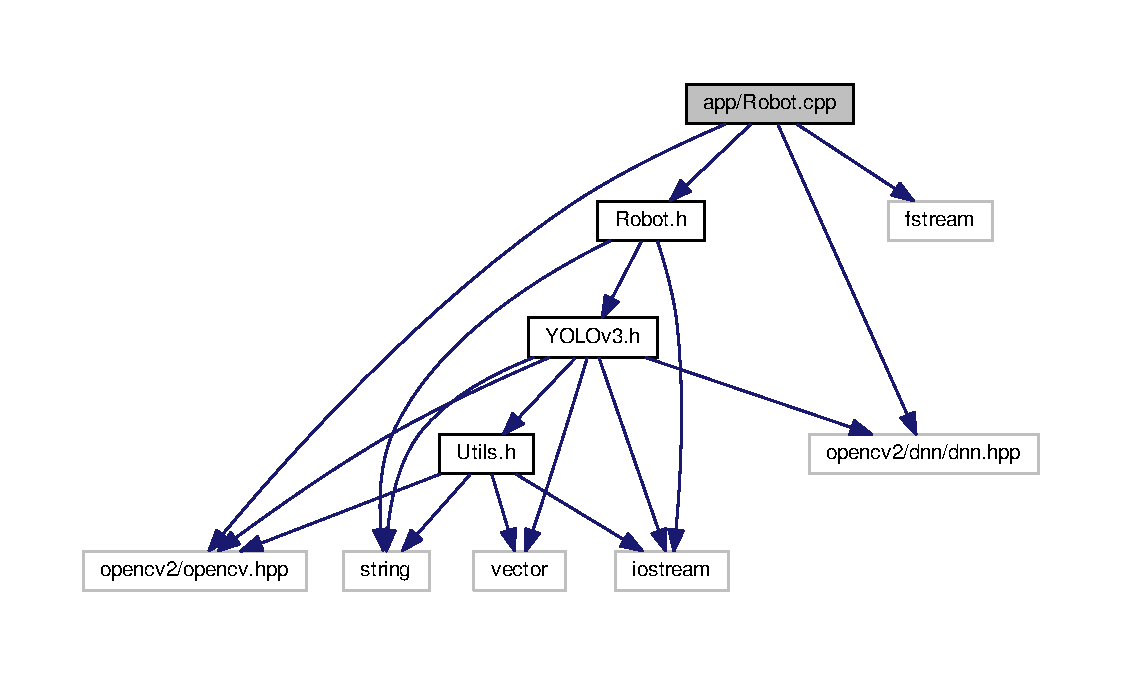
\includegraphics[width=350pt]{Robot_8cpp__incl}
\end{center}
\end{figure}


\subsection{Detailed Description}
Implementation for \hyperlink{classRobot}{Robot} class. 

\begin{DoxyCopyright}{Copyright}
M\+IT License (c) 2019 Arpit Aggarwal, Shantam Bajpai
\end{DoxyCopyright}
\begin{DoxyAuthor}{Author}
Arpit Aggarwal, Shantam Bajpai 
\end{DoxyAuthor}

\hypertarget{Utils_8cpp}{}\section{app/\+Utils.cpp File Reference}
\label{Utils_8cpp}\index{app/\+Utils.\+cpp@{app/\+Utils.\+cpp}}


Implementation for \hyperlink{classUtils}{Utils} class.  


{\ttfamily \#include $<$fstream$>$}\\*
{\ttfamily \#include \char`\"{}Utils.\+h\char`\"{}}\\*
{\ttfamily \#include $<$opencv2/opencv.\+hpp$>$}\\*
Include dependency graph for Utils.\+cpp\+:
\nopagebreak
\begin{figure}[H]
\begin{center}
\leavevmode
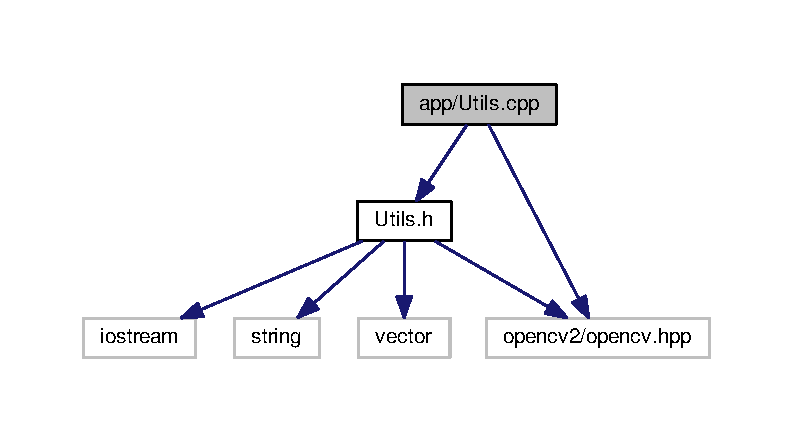
\includegraphics[width=350pt]{Utils_8cpp__incl}
\end{center}
\end{figure}


\subsection{Detailed Description}
Implementation for \hyperlink{classUtils}{Utils} class. 

\begin{DoxyCopyright}{Copyright}
M\+IT License (c) 2019 Arpit Aggarwal, Shantam Bajpai
\end{DoxyCopyright}
\begin{DoxyAuthor}{Author}
Arpit Aggarwal, Shantam Bajpai 
\end{DoxyAuthor}

\hypertarget{YOLOv3_8cpp}{}\section{app/\+Y\+O\+L\+Ov3.cpp File Reference}
\label{YOLOv3_8cpp}\index{app/\+Y\+O\+L\+Ov3.\+cpp@{app/\+Y\+O\+L\+Ov3.\+cpp}}


Implementation for \hyperlink{classYOLOv3}{Y\+O\+L\+Ov3} class.  


{\ttfamily \#include \char`\"{}Y\+O\+L\+Ov3.\+h\char`\"{}}\\*
{\ttfamily \#include $<$iterator$>$}\\*
{\ttfamily \#include $<$opencv2/opencv.\+hpp$>$}\\*
{\ttfamily \#include $<$opencv2/dnn/dnn.\+hpp$>$}\\*
Include dependency graph for Y\+O\+L\+Ov3.\+cpp\+:
\nopagebreak
\begin{figure}[H]
\begin{center}
\leavevmode
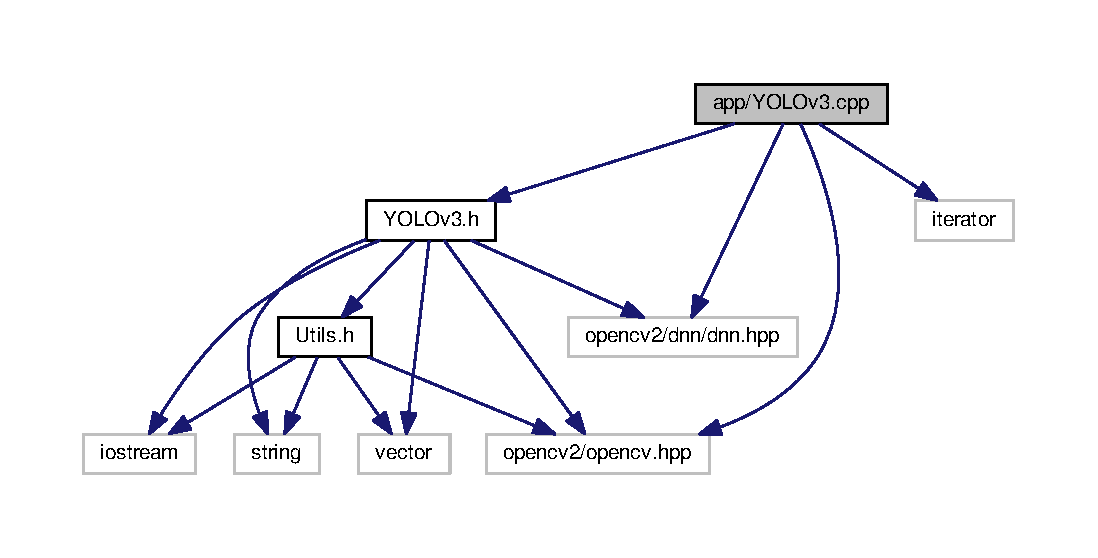
\includegraphics[width=350pt]{YOLOv3_8cpp__incl}
\end{center}
\end{figure}


\subsection{Detailed Description}
Implementation for \hyperlink{classYOLOv3}{Y\+O\+L\+Ov3} class. 

\begin{DoxyCopyright}{Copyright}
M\+IT License (c) 2019 Arpit Aggarwal, Shantam Bajpai
\end{DoxyCopyright}
\begin{DoxyAuthor}{Author}
Arpit Aggarwal, Shantam Bajpai 
\end{DoxyAuthor}

\hypertarget{test_8cpp}{}\section{test/test.cpp File Reference}
\label{test_8cpp}\index{test/test.\+cpp@{test/test.\+cpp}}


Test source file for enpm808x\+\_\+obstacle\+\_\+detector Contains the required headers and methods.  


{\ttfamily \#include $<$gtest/gtest.\+h$>$}\\*
{\ttfamily \#include $<$Robot.\+h$>$}\\*
{\ttfamily \#include $<$Utils.\+h$>$}\\*
{\ttfamily \#include $<$Y\+O\+L\+Ov3.\+h$>$}\\*
{\ttfamily \#include $<$vector$>$}\\*
Include dependency graph for test.\+cpp\+:
\nopagebreak
\begin{figure}[H]
\begin{center}
\leavevmode
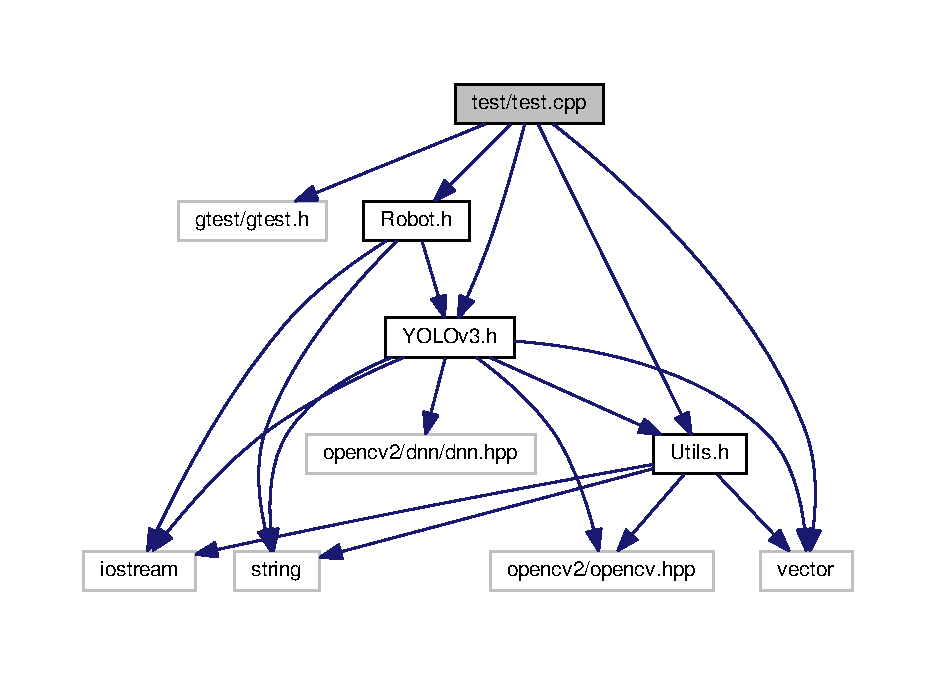
\includegraphics[width=350pt]{test_8cpp__incl}
\end{center}
\end{figure}
\subsection*{Functions}
\begin{DoxyCompactItemize}
\item 
\hyperlink{test_8cpp_a0b848d6666a4624da2e5e0f8029d4973}{T\+E\+ST} (check\+Getter\+Setter, check\+Conf\+Threshold)\hypertarget{test_8cpp_a0b848d6666a4624da2e5e0f8029d4973}{}\label{test_8cpp_a0b848d6666a4624da2e5e0f8029d4973}

\begin{DoxyCompactList}\small\item\em Test case for set\+Conf\+Threshold method of \hyperlink{classYOLOv3}{Y\+O\+L\+Ov3} class. The test checks whether value set for confidence is same as the value input by the get\+Conf\+Threshold method. \end{DoxyCompactList}\item 
\hyperlink{test_8cpp_a6f78ab2ce61f7fa291249adb64025820}{T\+E\+ST} (check\+Getter\+Setter, checknms\+Threshold)\hypertarget{test_8cpp_a6f78ab2ce61f7fa291249adb64025820}{}\label{test_8cpp_a6f78ab2ce61f7fa291249adb64025820}

\begin{DoxyCompactList}\small\item\em Test case for set\+Nms\+Threshold method of \hyperlink{classYOLOv3}{Y\+O\+L\+Ov3} class. The test checks whether value set for nms\+Threshold is same as the value input by the get\+Nms\+Threshold method. \end{DoxyCompactList}\item 
\hyperlink{test_8cpp_aba73f69ee75344002bf0a0fc6dea04e1}{T\+E\+ST} (check\+Getter\+Setter, check\+Input\+Width)\hypertarget{test_8cpp_aba73f69ee75344002bf0a0fc6dea04e1}{}\label{test_8cpp_aba73f69ee75344002bf0a0fc6dea04e1}

\begin{DoxyCompactList}\small\item\em Test case for set\+Input\+Width method of \hyperlink{classYOLOv3}{Y\+O\+L\+Ov3} class. The test checks whether value set for Input\+Width is same as the value input by the get\+Input\+Width method. \end{DoxyCompactList}\item 
\hyperlink{test_8cpp_a1d01c4edb3583b9a309a5770c4b86992}{T\+E\+ST} (check\+Getter\+Setter, check\+Input\+Height)\hypertarget{test_8cpp_a1d01c4edb3583b9a309a5770c4b86992}{}\label{test_8cpp_a1d01c4edb3583b9a309a5770c4b86992}

\begin{DoxyCompactList}\small\item\em Test case for set\+Input\+Height method of \hyperlink{classYOLOv3}{Y\+O\+L\+Ov3} class. The test checks whether value set for Input\+Height is same as the value input by the get\+Input\+Height method. \end{DoxyCompactList}\item 
\hyperlink{test_8cpp_a96de787502b2f7a44975352c13ed6ad2}{T\+E\+ST} (check\+Bool\+Setter\+Getter, check\+Is\+Image)\hypertarget{test_8cpp_a96de787502b2f7a44975352c13ed6ad2}{}\label{test_8cpp_a96de787502b2f7a44975352c13ed6ad2}

\begin{DoxyCompactList}\small\item\em Test case for get\+Is\+Image method of Foo class. The test checks whether the boolean value for get\+Is\+Image method. \end{DoxyCompactList}\item 
\hyperlink{test_8cpp_a9370048ababfebd67204034105355f66}{T\+E\+ST} (check\+Bool\+Setter\+Getter, check\+Is\+Video)\hypertarget{test_8cpp_a9370048ababfebd67204034105355f66}{}\label{test_8cpp_a9370048ababfebd67204034105355f66}

\begin{DoxyCompactList}\small\item\em Test case for get\+Is\+Video method of Foo class. The test checks whether the boolean value for get\+Is\+Image method. \end{DoxyCompactList}\item 
\hyperlink{test_8cpp_a704dabe6e3b7562d3c36e861b4a17e8f}{T\+E\+ST} (check\+Utils\+Getter\+Setter, check\+Classes\+File)\hypertarget{test_8cpp_a704dabe6e3b7562d3c36e861b4a17e8f}{}\label{test_8cpp_a704dabe6e3b7562d3c36e861b4a17e8f}

\begin{DoxyCompactList}\small\item\em Test case for get\+Classes\+File method of \hyperlink{classUtils}{Utils} class. \end{DoxyCompactList}\item 
\hyperlink{test_8cpp_ac18307310647ab7131ca17dc72a93cf8}{T\+E\+ST} (check\+Utils\+Getter\+Setter, check\+Model\+Configuration\+File)\hypertarget{test_8cpp_ac18307310647ab7131ca17dc72a93cf8}{}\label{test_8cpp_ac18307310647ab7131ca17dc72a93cf8}

\begin{DoxyCompactList}\small\item\em Test case for get\+Model\+Configuration method of \hyperlink{classUtils}{Utils} class. \end{DoxyCompactList}\item 
\hyperlink{test_8cpp_a06c1bda2499fc01d2fab12602d7cf45c}{T\+E\+ST} (check\+Utils\+Getter\+Setter, check\+Model\+Weights\+File)\hypertarget{test_8cpp_a06c1bda2499fc01d2fab12602d7cf45c}{}\label{test_8cpp_a06c1bda2499fc01d2fab12602d7cf45c}

\begin{DoxyCompactList}\small\item\em Test case for get\+Model\+Weights method of \hyperlink{classUtils}{Utils} class. \end{DoxyCompactList}\item 
\hyperlink{test_8cpp_a9b264885c85701d7b435738d0758206c}{T\+E\+ST} (check\+Utils\+Getter\+Setter, check\+Classes\+Size)\hypertarget{test_8cpp_a9b264885c85701d7b435738d0758206c}{}\label{test_8cpp_a9b264885c85701d7b435738d0758206c}

\begin{DoxyCompactList}\small\item\em Test case for get\+Classes method of \hyperlink{classUtils}{Utils} class. \end{DoxyCompactList}\end{DoxyCompactItemize}
\subsection*{Variables}
\begin{DoxyCompactItemize}
\item 
\hyperlink{classYOLOv3}{Y\+O\+L\+Ov3} {\bfseries yv3} (1, 1, 1, 1)\hypertarget{test_8cpp_a3a1fd8e840592ed3e69c6db83dbcdad4}{}\label{test_8cpp_a3a1fd8e840592ed3e69c6db83dbcdad4}

\item 
\hyperlink{classRobot}{Robot} {\bfseries f}\hypertarget{test_8cpp_a4a8e0921752ee80f8c8d17529a451b74}{}\label{test_8cpp_a4a8e0921752ee80f8c8d17529a451b74}

\item 
\hyperlink{classUtils}{Utils} {\bfseries Util}\hypertarget{test_8cpp_ab8e8d0e54cb77ebf75533c1b382c8a3e}{}\label{test_8cpp_ab8e8d0e54cb77ebf75533c1b382c8a3e}

\item 
double {\bfseries val} = 2\hypertarget{test_8cpp_a3c8bc0bb4f045bfe78d1196cb786792c}{}\label{test_8cpp_a3c8bc0bb4f045bfe78d1196cb786792c}

\item 
int {\bfseries val1}\hypertarget{test_8cpp_a948167f8090ebc248e42325a827e9371}{}\label{test_8cpp_a948167f8090ebc248e42325a827e9371}

\end{DoxyCompactItemize}


\subsection{Detailed Description}
Test source file for enpm808x\+\_\+obstacle\+\_\+detector Contains the required headers and methods. 

Copyright 2019 Shantam Bajpai and Arpit Aggarwal

\begin{DoxyAuthor}{Author}
Shantam Bajpai and Arpit Aggarwal 
\end{DoxyAuthor}
\begin{DoxyDate}{Date}
13th October 2019 
\end{DoxyDate}
\begin{DoxyVersion}{Version}
1.\+0 
\end{DoxyVersion}

%--- End generated contents ---

% Index
\backmatter
\newpage
\phantomsection
\clearemptydoublepage
\addcontentsline{toc}{chapter}{Index}
\printindex

\end{document}
